% A natural transformation α between two functors F, G : A → B,
% shown as arrows α_{A_i} between the F- and G-images of each object.
% Source: book/tex/cats/functors.tex (§ Natural transformations).
\documentclass[border=3mm]{standalone}
\usepackage{tikz}
\usetikzlibrary{arrows.meta}
\begin{document}
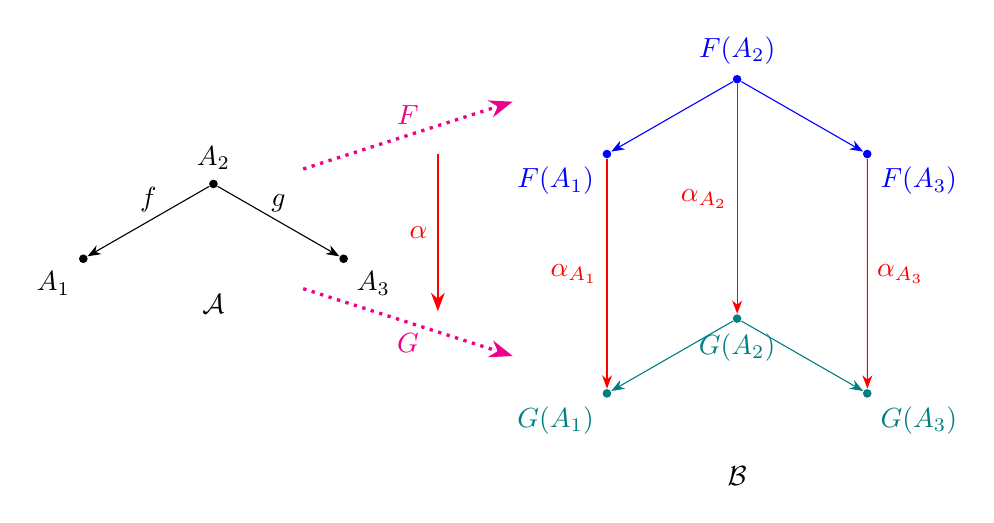
\begin{tikzpicture}[>=Stealth, scale=1.9, dot/.style={circle,fill,inner sep=1.1pt}]
  % Category A (left)
  \node[dot,label={below left:$A_1$}] (a1) at (-0.87,-0.5) {};
  \node[dot,label={above:$A_2$}] (a2) at (0,0) {};
  \node[dot,label={below right:$A_3$}] (a3) at (0.87,-0.5) {};
  \draw[->] (a2)--(a1) node[midway,above]{$f$};
  \draw[->] (a2)--(a3) node[midway,above]{$g$};
  \node at (0,-0.8) {$\mathcal A$};
  % F copy (blue)
  \node[dot,blue,label={[blue]below left:$F(A_1)$}] (f1) at (2.63,0.2) {};
  \node[dot,blue,label={[blue]above:$F(A_2)$}] (f2) at (3.5,0.7) {};
  \node[dot,blue,label={[blue]below right:$F(A_3)$}] (f3) at (4.37,0.2) {};
  \draw[->,blue] (f2)--(f1);
  \draw[->,blue] (f2)--(f3);
  % G copy (teal)
  \node[dot,teal,label={[teal]below left:$G(A_1)$}] (g1) at (2.63,-1.4) {};
  \node[dot,teal,label={[teal]below:$G(A_2)$}] (g2) at (3.5,-0.9) {};
  \node[dot,teal,label={[teal]below right:$G(A_3)$}] (g3) at (4.37,-1.4) {};
  \draw[->,teal] (g2)--(g1);
  \draw[->,teal] (g2)--(g3);
  % natural transformation alpha (red)
  \draw[->,red] (f1)--(g1) node[midway,left]{\color{red}$\alpha_{A_1}$};
  \draw[->,red] (f2)--(g2) node[midway,left]{\color{red}$\alpha_{A_2}$};
  \draw[->,red] (f3)--(g3) node[midway,right]{\color{red}$\alpha_{A_3}$};
  % F, G functor arrows (magenta dotted)
  \draw[->,magenta,dotted,very thick] (0.6,0.1)--(2.0,0.55) node[midway,above]{\color{magenta}$F$};
  \draw[->,magenta,dotted,very thick] (0.6,-0.7)--(2.0,-1.15) node[midway,below]{\color{magenta}$G$};
  % alpha between the two functors
  \draw[->,red,thick] (1.5,0.2)--(1.5,-0.85) node[midway,left]{\color{red}$\alpha$};
  \node at (3.5,-1.95) {$\mathcal B$};
\end{tikzpicture}
\end{document}
